% !TeX program = xelatex
\documentclass[landscape,a4paper]{ctexart}
\makeatletter
\def\input@path{{../../Templates/}}
\makeatother
\usepackage[opentypefonts]{zh-cheatsheet}
\usepackage{array}

% Match the Word edition, including bold Chinese and upright math operators.
\setCJKmainfont[AutoFakeBold=2]{Adobe Fangsong Std}
\setCJKsansfont[AutoFakeBold=2]{Adobe Fangsong Std}
\setCJKmonofont[AutoFakeBold=2]{Adobe Fangsong Std}
\setmathfont{Concrete-Math.otf}
\setoperatorfont\symup

% Common probability notation; use these commands in math mode.
\newcommand{\mean}[1]{\mathbb{E}\left[#1\right]}
\newcommand{\prob}[1]{\mathbb{P}\left\{#1\right\}}
\newcommand{\var}[1]{\operatorname{Var}\left[#1\right]}
% Mean-square convergence: \msconv or \msconv[t\to\infty].

\newcommand{\msconv}[1][]{\xrightarrow[#1]{\mathrm{m.s.}}}

% Two-column formula table: each row stays intact; the card may split between rows.
\newcommand{\msformulacells}[2]{%
  \noindent\begin{tabular}[t]{@{}>{\raggedright\arraybackslash}p{0.49\linewidth}@{\hspace{0.02\linewidth}}>{\raggedright\arraybackslash}p{0.49\linewidth}@{}}%
    #1 & #2
  \end{tabular}\par
}
\newcommand{\msformulasolidrule}[1]{%
  \par\nointerlineskip
  \noindent\makebox[\linewidth][l]{\color{black!70}\rule{\linewidth}{#1}}\par
  \nointerlineskip
}
\newcommand{\msformuladashrule}{%
  \par\nointerlineskip
  \noindent\makebox[\linewidth][l]{\hbox to\linewidth{\color{black!30}%
    \leaders\hbox{\rule{2pt}{0.25pt}\hskip1.5pt}\hfill}}\par
  \nointerlineskip
}
\newenvironment{msformula}{%
  \begin{array}[t]{@{}>{\displaystyle}l@{}}%
}{%
  \end{array}%
}
\newif\ifmsformulafirst
\newcommand{\msformularow}[2]{%
  \ifmsformulafirst
    \msformulafirstfalse
  \else
    \nobreak\vskip1.5pt\msformuladashrule
    \penalty0\vskip1.5pt
  \fi
  \msformulacells{#1}{#2}%
}
\newenvironment{msformulatable}{%
  \par\begingroup\renewcommand{\arraystretch}{1.0}%
  \msformulasolidrule{0.6pt}\nobreak\vskip2pt
  \msformulacells{\textbf{一般过程}}{\textbf{宽平稳过程}}%
  \nobreak\vskip2pt\msformulasolidrule{0.4pt}\nobreak\vskip2pt
  \msformulafirsttrue
}{%
  \par\nobreak\vskip2pt\msformulasolidrule{0.6pt}%
  \endgroup\par
}



% Use ragged-right alignment for card text and titles.
\tcbset{halign=flush left,halign title=flush left}
% Reserve the full column remainder for non-final pieces of a split card.
% This keeps tcolorbox's height estimate in sync with multicols*.
\tcbset{height fixed for=first and middle}

\begin{document}
\raggedright
	\begin{cheatsheetcolumns}
		\begin{card}{随机过程概念}
			\begin{itemize}
				\item 随机过程：带时间的一列随机变量
				\begin{itemize}
					\item \textbf{集合}视角：定义在样本空间$\left(\Omega,\mathcal{F}, P\right)$上的随机过程族$\left\{X(t_1), X(t_2), \dots\colon t_1, t_2, \dots \in T\right\}$ 
					\item \textbf{映射}视角：$X\colon T\times \Omega\to \mathbb{R}$；$\left(t,\omega\right)\mapsto X(t, \omega)$
				\end{itemize}
					\item 随机过程的数字特征
					\begin{itemize}
						\item \textbf{均值}：$\mu_X(t)=\mean{X(t)}=\int_{-\infty}^{+\infty}xf(x;t)\,\mathrm{d}x$
						\item \textbf{方差}：$\var{X(t)}=\mean{\left\lvert X(t)\right\rvert^2}-\left\lvert\mean{X(t)}\right\rvert^2$
						\item \textbf{自相关}：$R_{X}(t_1, t_2)=\mean{X(t_1)X^\ast(t_2)}$
						\item \textbf{互相关}：$R_{XY}(t_1, t_2)=\mean{X(t_1)Y^\ast(t_2)}$
						\item \textbf{（自）协方差}：$C_{XY}(t_1, t_2)=\mean{X(t_1)Y^\ast(t_2)}-\mean{X(T_1)}\mean{Y^\ast(t_2)}$
					\end{itemize}
					\item 随机等价：\par
						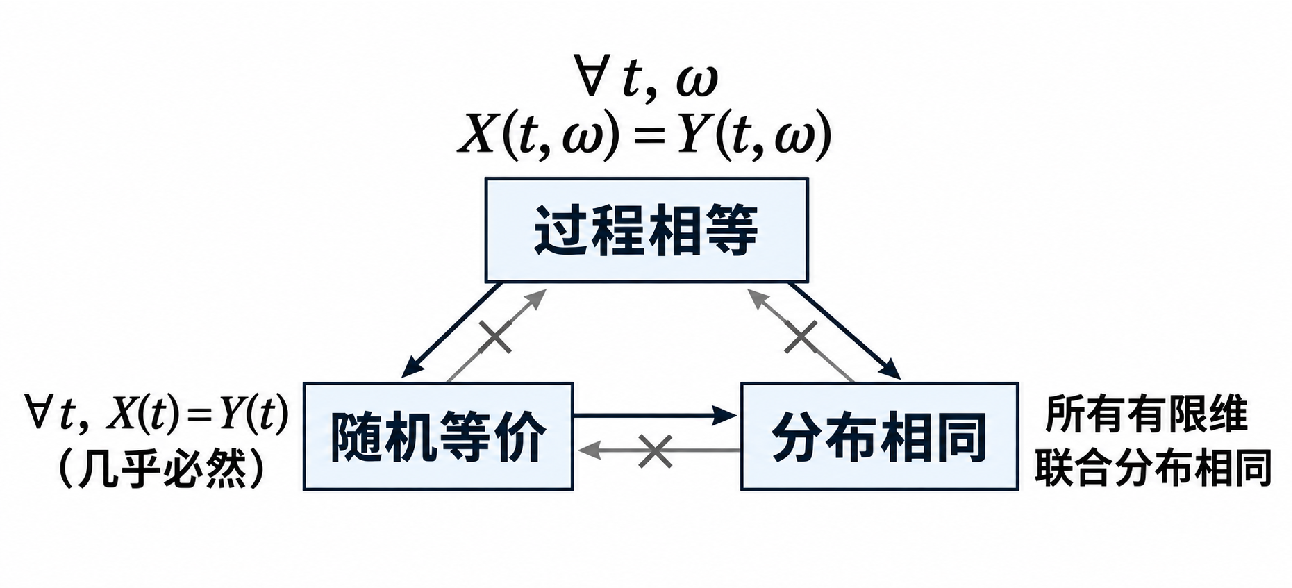
\includegraphics[width=.6\linewidth]{stochastic_equivalence_flat.pdf}
					\item 向量随机过程：一列随机过程组成的向量 $\mathbf{X}(t)=\left(X_1(t), X_2(t), \dots\right)^\intercal$
					\begin{itemize}
						\item \textbf{均值}：$\mu_{\mathbf X}(t)=\left(\mean{X_1(t)}, \mean{X_2(t)},\dots\right)^\intercal$
						\item \textbf{自相关矩阵}：$\mathbf{R}_{\mathbf{X}}(t_1, t_2)=\mean{\mathbf{X}(t_1)\mathbf{X}(t_2)^{\mathrm{H}}}$
						\item \textbf{互相关矩阵}：$\mathbf{R}_{\mathbf{X}\mathbf{Y}}(t_1, t_2)=\mean{\mathbf{X}(t_1)\mathbf{Y}(t_2)^{\mathrm{H}}}$ 
						\item \textbf{（自）协方差矩阵}：$\mathbf{C}_{\mathbf{X}\mathbf{Y}}(t_1, t_2)=\mean{\mathbf{X}(t_1)\mathbf{Y}(t_2)^{\mathrm{H}}}-\mean{\mathbf{X}(t_1)}\mean{\mathbf{Y}(t_2)}^{\mathrm{H}}$ 
					\end{itemize}
			\end{itemize}
		\end{card}
		\begin{card}{随机过程的平稳性}
			\begin{itemize}
				\item 内积不等式：将随机变量的互相关 $R_{XY}=\mean{XY^\ast}$ 视作内积，
				\[\left\lvert\mean{XY^\ast}\right\rvert^2\le \mean{\left\lvert X\right\rvert^2}\mean{\left\lvert Y\right\rvert^2}
				\]
				等号成立 $\Leftrightarrow$ $X$ 和 $Y$ 几乎必然线性相关
				\item 自相关函数性质：
				\begin{itemize}
					\item 共轭对称性：$R_X(t_1, t_2)=R_X^\ast(t_2, t_2)$
					\begin{itemize}
						\item （向量）自相关矩阵共轭对称：
						$
						\mathbf{R}_{\mathbf{X}}=\mathbf{R}_{\mathbf{X}}^{\mathrm{H}}
						$
					\end{itemize}
					\item 非负定性：\textbf{有限时刻自相关矩阵}非负定\\
					令$\mathbf{Z}=(X(t_1),\ldots,X(t_n))^\intercal$，$\mathbf{R}_X[t_1,\ldots,t_n]=\mathbb{E}[\mathbf{Z}\mathbf{Z}^{\mathsf{H}}]$非负定
				\end{itemize}
				\item \textbf{宽平稳}：随机过程的\textbf{均值}不随时间变化，\textbf{自相关函数}只与两时刻之差有关
				\[
				\mean{X(t)}=\mu,\qquad R_X(t_1, t_2)=R_X(\tau)(\tau=t_2-t_1)
				\]
				\begin{itemize}
					\item 自相关函数共轭对称：$R_X(\tau)=R^\ast(-\tau)$
					\item 自相关在$\tau=0$处取最大值：$\left|R_X(\tau)\right|\le R_X(0)$
					\item 协方差在$\tau=0$处取最大值：$\left|C_X(\tau)\right|\le C_X(0)=\var{X(t)}$
					\item 相关系数$r_X(\tau)=\frac{C_X(\tau)}{C_X(0)}$，相关时间$\tau_0=\int_0^{+\infty}r_X(\tau)\,\mathrm{d}\tau$
				\end{itemize}
				\item 联合宽平稳：两宽平稳过程$X(t)$，$Y(t)$满足
				\[
				R_{XY}(t,s)=R_{XY}(t+\tau, s+\tau)
				\]
				\item \textbf{随机变量的关系}：
				\begin{itemize}
					\item 正交：$R_{XY}=\mean{XY^\ast}=0$
					\item 不相关：$\operatorname{Cov}(X,Y)=R_{XY}-\mean{X}\mean{Y^\ast}=0$
					\item 独立：
					$p_{X,Y}(x,y)=p_X(x)p_Y(y)$
					\item 独立必然不相关，反之不一定
				\end{itemize}
				\item 增量随机过程：$\forall t_1<t_2\le t_3 < t_4$\\增量$\Delta X(t_m, t_n)=X(t_n)-X(t_m)$
				\begin{itemize}
					\item 正交增量过程：$\Delta X(t_1, t_2)$与$\Delta X(t_3, t_4)$ 正交
					\item 独立增量过程：$\Delta X(t_1, t_2)$与$\Delta X(t_3, t_4)$ 独立
					\item 平稳增量过程：$\Delta X(t_m, t_n)$只取决于$t_n-t_m$
				\end{itemize}
			\end{itemize}
		\end{card}
		\begin{card}{导数和积分}
			\begin{itemize}
				\item \textbf{均方收敛}：若二阶矩过程$X(t)$和随机变量$X$满足\[\lim_{t\to t_0}\mean{\left| X(t)-X\right|^2}=0\]则$X(t)$均方收敛于$X$（$X(t)\msconv X$）
				\item 柯西判别法：\\$X(n)$均方收敛$\Leftrightarrow\mean{\left|X(n)-X(m)\right|^2}\to 0$\hfill（$m,n\to \infty$）\\
				\item 洛伊夫判别法：\\$X(n)$均方收敛$\Leftrightarrow\mean{X(n)X^\ast(m)}\to C$\hfill（$m,n\to \infty$）
				\item \textbf{均方导数}：\\$\left(X(t+h)-X(t)\right)/h\msconv Y(t), t\in T, h\to 0$，则$X'(t)=Y(t)$
				\item \textbf{均方导数判定定理}：
				\begin{itemize}
					\item 若$\left.\pdv{R_X}!{u,v}(u, v)\right|_{(t, t)}$存在，则$X(t)$在$t$时刻可导
					\item 对于宽平稳过程：
					\begin{itemize}
						\item 宽平稳过程在某一时刻可导，则在任意时刻可导
						\item 宽平稳过程的导过程均方连续
						\item 宽平稳过程$X(t)$可导$\Leftrightarrow R_X''(0)$存在且有限
					\end{itemize}
			\end{itemize}
			\item \textbf{均方导数性质}：
			\begin{itemize}
				\item 线性：$\left(aX+bY\right)'=aX'+bY'$
				\item 
				\begin{itemize}
					\item \(X,Y\) \textbf{联合宽平稳}时，线性组合及其导过程均宽平稳
				\end{itemize}
				\item $\mean{X'(t)}=\odv{\mean{X(t)}}/{t}$
				\item $R_{X'Y}(t,s)=\pdv{R_{XY}(t,s)}!{t}$
				\item $R_{X'Y'}(t,s)=\pdv{R_{XY}(t,s)}!{t,s}$
				\item 宽平稳过程 $R_{X'}(\tau)=-R''_{X}(\tau)$
				\item $\left(f(t)X(t)\right)'=f'(t)X(t)+f(t)X'(t)$
			\end{itemize}
			\item \textbf{均方导数计算公式}：\\
			以下假设相应导数存在；一般相关函数省略$(t_1,t_2)$，沿用$\tau=t_2-t_1$。
			\begin{msformulatable}
			\msformularow{
				$\mean{X'(t)}=\mu_X'(t)$
			}{
				$\mean{X'(t)}=0$
			}
			\msformularow{
				$R_{X'X}=\pdv{R_X}!{t_1}$
			}{
				$R_{X'X}(\tau)=-R_X'(\tau)$
			}
			\msformularow{
				$R_{XX'}=\pdv{R_X}!{t_2}$
			}{
				$R_{XX'}(\tau)=R_X'(\tau)$
			}
			\msformularow{
				$R_{X'}=\pdv{R_X}!{t_1,t_2}$
			}{
				$R_{X'}(\tau)=-R_X''(\tau)$
			}
			\msformularow{
				$C_{X'}=\pdv{C_X}!{t_1,t_2}$
			}{
				$\begin{msformula}
					C_{X'}(\tau)=-C_X''(\tau)\\
					=R_{X'}(\tau)
				\end{msformula}$
			}
			\msformularow{
				$\begin{msformula}
					\var{X'(t)}\\
					{}=\left.\pdv{C_X}!{t_1,t_2}\right|_{t_1=t_2=t}
				\end{msformula}$
			}{
				$\var{X'(t)}=-R_X''(0)$
			}
			\msformularow{
				$\begin{msformula}
					\operatorname{Re}C_{XX'}(t,t)\\
					{}=\frac12\odv{\var{X(t)}}!{t}
				\end{msformula}$
			}{
				$\operatorname{Re}C_{XX'}(0)=0$\par
				实值时：$C_{XX'}(0)=0$
			}
			\msformularow{
				$\begin{msformula}
					\mean{|X(t+h)-X(t)|^2}\\
					{}=h^2\mean{|X'(t)|^2}\\
					{}+o(h^2)
				\end{msformula}$
			}{
				$\begin{msformula}
					2[R_X(0)-\operatorname{Re}R_X(h)]\\
					{}=-R_X''(0)h^2+o(h^2)
				\end{msformula}$
			}
			\msformularow{
				$\begin{msformula}
					R_{X^{(p)}X^{(q)}}\\
					{}=\frac{\partial^{p+q}R_X}{\partial t_1^p\,\partial t_2^q}
				\end{msformula}$
			}{
				$\begin{msformula}
					R_{X^{(p)}X^{(q)}}(\tau)\\
					{}=(-1)^pR_X^{(p+q)}(\tau)
				\end{msformula}$
			}
			\msformularow{
				$\begin{msformula}
					\var{X^{(n)}(t)}\\
					{}=\left.\frac{\partial^{2n}C_X}{\partial t_1^n\,\partial t_2^n}\right|_{t_1=t_2=t}
				\end{msformula}$
			}{
				$\begin{msformula}
					\var{X^{(n)}(t)}\\
					{}=(-1)^nR_X^{(2n)}(0)
				\end{msformula}$
			}
			\msformularow{
				无通用的平稳谱公式
			}{
				$S_{X^{(n)}}(\omega)=\omega^{2n}S_X(\omega)$
			}
			\msformularow{
				$\begin{msformula}
					\left(f(t)X(t)\right)'\\
					{}=f'(t)X(t)+f(t)X'(t)
				\end{msformula}$
			}{
				一般不平稳
			}
			\msformularow{
				$\begin{msformula}
					\left(X(\phi(t))\right)'\\
					{}=\phi'(t)X'(\phi(t))
				\end{msformula}$
			}{
				$\begin{msformula}
					Y(t)=X(at+b)\\
					R_{Y'}(\tau)=-a^2R_X''(a\tau)
				\end{msformula}$
			}
			\end{msformulatable}
			其中$n\ge1$；谱公式假设谱密度存在，$\omega$为角频率。
			\item 若随机过程$\xi(t)=f(t, T)$，其中$T$是随机变量，则
			\[
			\odv{\xi(t)}{t}=\pdv{f(t,T)}{t},\quad \int_a^b \xi(t)\,\mathrm dt=\int_a^b f(t,T)\,\mathrm dt
			\]
			\end{itemize}
			
		\end{card}
	\end{cheatsheetcolumns}
\end{document}
